\documentclass[5p,times]{elsarticle}

% INS-oriented two-column draft. The abstract is intentionally deferred.
\usepackage[utf8]{inputenc}
\usepackage[T1]{fontenc}
\usepackage{lmodern}
\usepackage{amsmath,amssymb,booktabs,tabularx,multirow}
\usepackage{graphicx}
\usepackage{xcolor}
\usepackage{tikz}
\usetikzlibrary{positioning}
\usepackage{pgfplots}
\pgfplotsset{compat=1.18}
\usepackage{enumitem}
\usepackage{microtype}
\usepackage{balance}
\usepackage{hyperref}
\hypersetup{hidelinks}

\newcolumntype{L}[1]{>{\raggedright\arraybackslash}p{#1}}
\setlength{\emergencystretch}{1em}

\journal{Information Sciences}

\newcommand{\admissible}{\mbox{\textsc{Admissible}}}
\newcommand{\reject}{\mbox{\textsc{Reject}}}
\newcommand{\primary}{\mbox{\textsc{Primary}}}
\newcommand{\todo}[1]{\textcolor{red}{[TODO: #1]}}

\begin{document}

\begin{frontmatter}

\title{When Candidate Retrieval Is Not Admission: A Coverage-Aware Diagnostic Benchmark for Open-Web Event Organization}

\author[inst1]{Anonymous authors}
\address[inst1]{Under double-blind review}

% Abstract intentionally deferred for the next writing pass.
\begin{abstract}
\todo{Write the abstract after the main argument and all claims have been finalized.}
\end{abstract}

\begin{keyword}
event linking \sep open-world information extraction \sep benchmark \sep calibration \sep selective prediction \sep information processing
\end{keyword}

\end{frontmatter}

\section{Introduction}
\label{sec:intro}

An event-linking system normally receives an input that is already assumed to express an event. It then decides whether the mention links to a known event or should be assigned a NIL-like outcome. That assumption is useful for studying entity resolution, but it is not neutral when the output is consumed by an event organization system. Open-web inputs often contain people, places, topics, or local actions without foregrounding an event that should be inserted into an event timeline. Treating every retrieved candidate as evidence that the whole item is admissible therefore conflates several decisions that occur at different levels.

This paper began with a recurring observation in an EventLink-NYT audit: many inputs that produced plausible candidate mentions were not suitable for downstream event organization under a fixed editorial policy. The observation was not that these inputs were false, nor that they were all non-events. The narrower and operational question was whether the item should enter an event organization pipeline given the available evidence. This distinction led us to separate three units: a mention supplied to a linker, a target returned by retrieval, and an item-level admission decision. In particular, an item-level \reject{} is not the same label as an out-of-knowledge-base event (a NEW or NIL-EVENT case).

The distinction matters because the usual score-only view can hide failures before a score exists. A system may retrieve no candidate, produce an invalid span, or fail to return a legal structured response. These cases are not harmless implementation noise when the deployed action is admission. They change the denominator of the operational decision. Conversely, a system with excellent ranking discrimination can still admit too many \reject{} items at a fixed operating point. A benchmark that reports only AUC on rows with valid scores cannot expose this interaction.

We therefore develop a compact, coverage-aware diagnostic benchmark for \emph{open-web event admission}. The benchmark does not introduce a new event-linking architecture. Instead, it makes the admission contract explicit and evaluates a frozen candidate-to-admission chain using item-level denominators. The protocol records candidate coverage, parsing and generation failures, Admission Retention, and \reject{} false-acceptance rate (FAR), in addition to conventional ranking metrics. Development material is kept separate from a new-time-window challenge confirmation set, and all methods are evaluated once under thresholds selected before the confirmation labels are opened.

The final result is intentionally not a leaderboard claim. On the new-time-window set, the frozen joint primary system has 79/102 score coverage and retains 40/57 \admissible{} items at 10/45 \reject{} false admissions. A direct admission baseline has complete coverage and retains 46/57 at the same number of false admissions. The paired uncertainty interval does not establish a statistically confirmed advantage for either system. The stable finding is instead that candidate coverage and calibration transfer are part of the admission problem: development-stage gains do not automatically survive a time-shifted input stream.

Our contributions are:
\begin{enumerate}[leftmargin=*,itemsep=2pt]
  \item a task definition that distinguishes mention, target, and item-level admission, while keeping \reject{} separate from NEW/NIL-EVENT;
  \item a measurement contract that decomposes candidate extraction, retrieval, eligibility, and admission and treats coverage and failures as first-class outcomes;
  \item a layered benchmark design with task-unit calibration, controlled development diagnostics, and a non-overlapping time-window challenge confirmation set;
  \item an empirical analysis showing that a frozen joint signal does not establish a general advantage over direct admission, and that missing candidates and parsing failures materially affect the measured result.
\end{enumerate}

The paper is deliberately scoped as a diagnostic benchmark and protocol study. We do not estimate Web prevalence, claim complete EXISTING/NEW/REJECT linking, or argue that a new model family is necessary. Those boundaries make the negative result informative rather than a failed attempt to force a method contribution.

\section{Related Work}
\label{sec:related}

Event linking has traditionally been formulated around a detected event mention and a decision to ground it to a knowledge-base entry or return a NIL-like outcome. Recent work has improved grounding to Wikipedia and has incorporated argument-aware evidence, but these formulations still operate at the mention/target interface rather than defining an item-level admission contract \citep{eventlinking2023,argumentaware2024}. Selective entity-linking work has likewise shown that a system can learn when not to link, but the abstention decision is not identical to deciding whether an upstream item should enter event organization \citep{learnnotlink2023}.

Our contribution is therefore complementary to NIL prediction. We retain the useful distinction between known and unknown targets, while adding an explicit operational state for inputs that do not satisfy the admission policy. The methodological focus is evaluation: a candidate-centric score is insufficient when candidate coverage and parsing failures determine whether an item can be scored at all. The benchmark is intended as a protocol for comparing future models, not as a replacement for existing event-linking tasks.

\section{From the Observed Phenomenon to a Measurable Task}
\label{sec:phenomenon}

\subsection{The initial audit}

The Stage1 audit reconstructed 639 unique released texts from 993 EventLink-NYT NIL mention rows. An operational overlay contained 599 EVENT-DESCRIBABLE items and 40 \reject{} items. The resulting conditional estimate was 6.78\%, with a finite-population interval of 6.26--9.39\%. This number describes a screened EventLink candidate pool; it is not an estimate of the natural \reject{} rate on the open Web. The same audit showed that the 40 item labels corresponded to 62 original candidate mentions, making it unsafe to copy mention-level labels into an item-level three-way link Gold.

The qualitative boundary was consistent across difficult cases. A post could contain a named person, a location, or an action phrase while using the rest of the text for personal narrative, background, or scene description. Such a post could be meaningful and factually true but still fail the policy for entering an event organization workflow. The observation motivated a separate admission state, not a stronger assertion about whether an event exists in the world.

\subsection{Units and operational labels}

Let $x_i$ denote an input item, $m_{ij}$ its extracted mentions, and $t_{ijk}$ a retrieved target candidate. The benchmark records labels at the item level:
\begin{equation}
 y_i \in \{\admissible{},\reject{}\}.
\end{equation}
An \admissible{} item may have one or more candidates, while a \reject{} item may also have plausible candidates. The label means ``admit under the frozen evidence policy'', not ``an event does not exist'' and not ``the target is outside the knowledge base''. This distinction is central to the benchmark's validity.

We evaluate the following chain:
{\small
\begin{equation}
 x_i \xrightarrow{\text{candidate extraction}} M_i
 \xrightarrow{\text{retrieval}} T_i
 \xrightarrow{\text{eligibility}} S_i
 \xrightarrow{\text{admission}} \hat y_i.
\end{equation}
}
Each arrow can fail. The benchmark consequently reports an item in the denominator even when $M_i$, $T_i$, or $S_i$ is missing. A missing score is an abstention/non-admission operationally; it is not converted into an artificial numeric score.

\begin{figure*}[t]
  \centering
  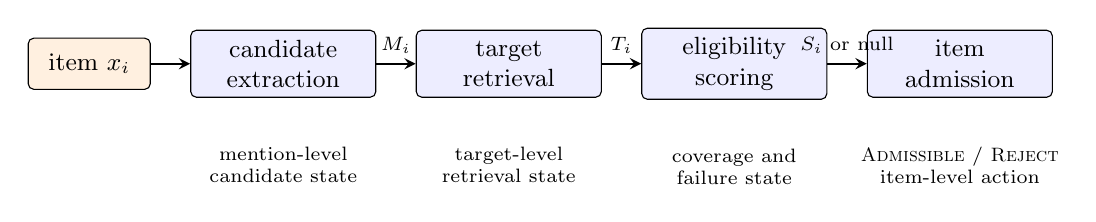
\begin{tikzpicture}[font=\small, node distance=7mm and 5mm, >=stealth]
  \tikzstyle{stage}=[draw, rounded corners=2pt, minimum width=2.35cm, minimum height=0.85cm, align=center, fill=blue!7]
  \tikzstyle{unit}=[draw, rounded corners=2pt, minimum width=1.55cm, minimum height=0.65cm, align=center, fill=orange!12]
  \node[unit] (item) {item $x_i$};
  \node[stage, right=of item] (extract) {candidate\\extraction};
  \node[stage, right=of extract] (retrieve) {target\\retrieval};
  \node[stage, right=of retrieve] (elig) {eligibility\\scoring};
  \node[stage, right=of elig] (admit) {item\\admission};
  \draw[->, thick] (item) -- (extract);
  \draw[->, thick] (extract) -- node[above, font=\scriptsize] {$M_i$} (retrieve);
  \draw[->, thick] (retrieve) -- node[above, font=\scriptsize] {$T_i$} (elig);
  \draw[->, thick] (elig) -- node[above, font=\scriptsize] {$S_i$ or null} (admit);
  \node[below=5mm of extract, align=center, font=\scriptsize] {mention-level\\candidate state};
  \node[below=5mm of retrieve, align=center, font=\scriptsize] {target-level\\retrieval state};
  \node[below=5mm of elig, align=center, font=\scriptsize] {coverage and\\failure state};
  \node[below=5mm of admit, align=center, font=\scriptsize] {$\admissible{}$ / $\reject{}$\\item-level action};
\end{tikzpicture}

  \caption{The measured decision chain. Mention-level candidate extraction and target retrieval are upstream signals; item-level admission is the downstream action. The benchmark keeps their units and failure states separate.}
  \label{fig:pipeline}
\end{figure*}

\section{Benchmark Design and Evidence Hierarchy}
\label{sec:benchmark}

\subsection{Evidence layers}

The materials were selected for different evidential jobs rather than pooled into one nominally large test set. Table~\ref{tab:data} records the separation used in all analyses.

\begin{table*}[t]
\centering
\caption{Evidence layers and their role. Identical item sets are not counted twice.}
\label{tab:data}
\footnotesize
\setlength{\tabcolsep}{4pt}
\renewcommand{\arraystretch}{1.08}
\begin{tabularx}{\textwidth}{@{}L{0.12\textwidth} L{0.30\textwidth} L{0.18\textwidth} X@{}}
\toprule
Layer & Size and labels & Evidence status & Role and boundary \\
\midrule
P0 calibration & 80 items, 124 mentions; 39 YES, 39 NO, 2 UNCERTAIN & Development & Aligns mention, target, and item units. Not a system test or NEW Gold. \\
DEV30 & 30 items & Development & Selects operating points and supports method development. Never used as independent confirmation. \\
EVAL60 / Web60 & 60 items; 33 \admissible{}, 27 \reject{} & Controlled diagnostic & Same item set as EVAL60; original A/B agreement 51/60, $\kappa=.6932$. Not prevalence or untouched test data. \\
D2 challenge & 102 new items; 57 \admissible{}, 45 \reject{} & Challenge confirmation & Bluesky AppView, fixed queries and new time window; zero overlap with 1,029 historical records under the frozen audit. Not a probability sample. \\
\bottomrule
\end{tabularx}
\end{table*}

P0 was used to prevent accidental propagation of old mention-level EventLink labels into an item-level Gold. DEV30 and EVAL60 support controlled comparisons; candidate recovery and clean shallow controls reuse the same 90 items. D2 is the only new-time-window confirmation material. The 300-item capped retrieval pool and the historical 1,762 mention rows remain useful provenance and diagnostic material, but are not silently promoted to the same item-level test population.

\subsection{D2 challenge confirmation}

D2 contains 102 items collected through Bluesky Public AppView searchPosts between 2026-09-22 and 2026-09-28 UTC using 12 fixed English topic queries. Historical overlap checks covered exact source IDs, normalized bodies, external URLs, near duplicates, and content clusters; all were zero. The two blind packages contained the same content in independently randomized order and exposed only text, time, and reply/quote/media metadata. No label, candidate, score, model output, or recommendation was shown during A/B annotation.

The first complete submissions agreed on 85/102 items ($83.33\%$, Cohen's $\kappa=.6612$). Seventeen disagreements were adjudicated by a human C pass, resulting in 57 \admissible{} and 45 \reject{} labels. Human adjudication used a machine-translation aid for some English text; this is disclosed as provenance and is not described as a third independent annotator. D2 is a controlled-calibration challenge set, not a probability sample and not a Web prevalence estimate.

\section{Experimental Protocol}
\label{sec:protocol}

\subsection{Frozen methods}

The one-pass D2 evaluation included eight frozen methods: BM25 top-1 retrieval, BGE top-1 retrieval, a validity score, direct admission, clean linear and RBF controls, the original exact-existing joint-linear system (the \primary{}), and an admit-all reference. Thresholds and model choices were fixed from DEV material. D2 labels were not used for prompt, feature, threshold, or hyperparameter selection.

The protocol required every D2 item to remain in the audit denominator. Legal statuses included \texttt{OK}, \texttt{NO\_CANDIDATE}, \texttt{INVALID\_JSON}, \texttt{INVALID\_SPANS}, and other named failure states. Missing or non-finite scores remained null and were reported as abstention; no zero or sentinel score was substituted.

\subsection{Metrics}

For Gold class $c$, Admission Retention and \reject{} FAR are:
{\small
\begin{equation}
 \begin{aligned}
 \mathrm{Retention}&=\frac{\#\{i:y_i=\admissible{},\ \hat y_i=\admissible{}\}}{\#\{i:y_i=\admissible{}\}},\\
 \mathrm{FAR}_{R}&=\frac{\#\{i:y_i=\reject{},\ \hat y_i=\admissible{}\}}{\#\{i:y_i=\reject{}\}}.
 \end{aligned}
\end{equation}
}
Coverage is reported separately and never used to remove an item from either denominator. Full-set ROC-AUC and AUPRC are reported only when all 102 items have valid scores. Otherwise the full-set value is \nolinkurl{NA_NOT_FULL_COVERAGE}; a conditional AUC is labelled as such and cannot replace it. Intervals use the frozen 2,000-draw paired bootstrap, stratified by Gold class and content-cluster units. They describe the challenge set only.

\subsection{Reproducibility contract}

Before inference, the D2 package, system lock, runner, prompts, thresholds, knowledge base, and prepared input were hashed. Predictions were frozen before the Gold was opened. F2 then scored the frozen predictions once, followed by an independent replay verification. F3 rechecked IDs, class denominators, all eight metrics, curves, bootstrap intervals, and input/output hashes. After scoring, a read-only Gold hash was recomputed during hash registration; this exceeded the strict score-only access boundary but did not parse labels, alter predictions, or rerun scoring. We report this protocol deviation explicitly.

\section{Results}
\label{sec:results}

\subsection{Controlled development diagnostics}

On the controlled DEV30/EVAL60 material, the original EVAL60 AUCs were .7632 for BM25, .5466 for BGE, .7357 for validity, .7469 for direct admission, .7969 for the joint linear score, and .8058 for the joint RBF score. The joint linear system retained 19/33 \admissible{} items and falsely admitted 3/27 \reject{} items at its frozen operating point. These numbers establish that some signals are predictive in the controlled material; they do not establish an independent result because the set was used during development and adjudication.

\subsection{Challenge-set results}

Table~\ref{tab:main-results} gives the complete D2 denominator. Primary coverage is 79/102, so its full-set AUC and AUPRC are not estimable under the protocol. The conditional values are retained only as diagnostics.

\begin{table*}[t]
\centering
\caption{Fixed D2 evaluation on 102 items. Retention uses all 57 \admissible{} items; FAR uses all 45 \reject{} items. `NA' is required when score coverage is below 102/102.}
\label{tab:main-results}
\small
\begin{tabular}{@{}lrrrrl@{}}
\toprule
Method & Score coverage & Retained / 57 & False admitted / 45 & ROC-AUC & AUPRC \\
\midrule
Admit-all reference & 102/102 & 57 & 45 & .500 & .559 \\
BM25 top-1 & 101/102 & 53 & 27 & NA (cond. .741) & NA (cond. .747) \\
BGE top-1 & 101/102 & 55 & 40 & NA (cond. .672) & NA (cond. .723) \\
Validity & 79/102 & 44 & 13 & NA (cond. .870) & NA (cond. .894) \\
Direct admission & 102/102 & 46 & 10 & .868 & .902 \\
Clean linear & 102/102 & 39 & 24 & .526 & .546 \\
Clean RBF & 102/102 & 35 & 9 & .793 & .831 \\
\primary{} joint linear & 79/102 & 40 & 10 & NA (cond. .770) & NA (cond. .822) \\
\bottomrule
\end{tabular}
\end{table*}

The headline result is not that Direct admission wins. Its paired difference interval against Primary crosses zero, so a statistically confirmed overall advantage cannot be claimed. The stronger and safer observation is operational: at the same observed number of false admissions (10/45), Direct admission retains 46/57 items while Primary retains 40/57, and Direct has complete score coverage. The frozen joint signal therefore does not establish a general advantage over a direct baseline on the new time window.

\begin{figure}[t]
  \centering
  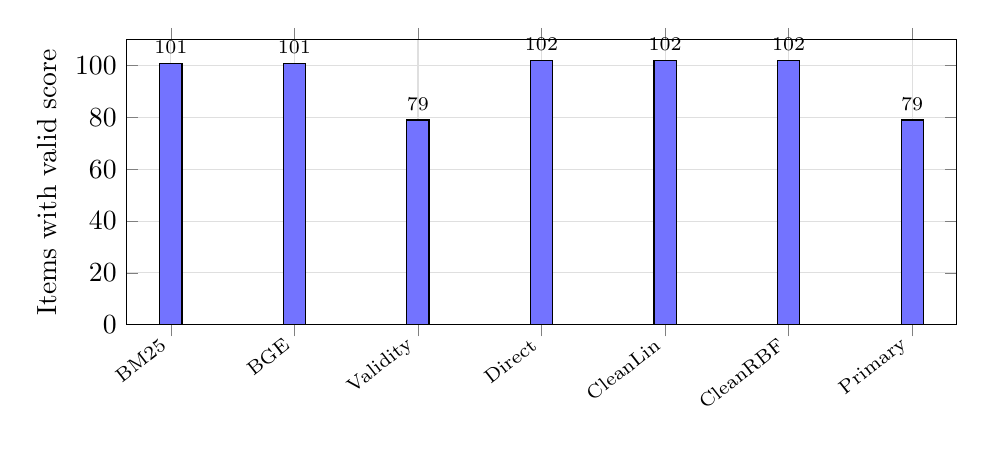
\begin{tikzpicture}
\begin{axis}[
  ybar, bar width=8pt, width=\columnwidth, height=5.2cm,
  ymin=0, ymax=110, ylabel={Items with valid score},
  symbolic x coords={BM25,BGE,Validity,Direct,CleanLin,CleanRBF,Primary},
  xtick=data, x tick label style={rotate=38,anchor=east,font=\scriptsize},
  ytick={0,20,40,60,80,100}, grid=major, major grid style={draw=gray!25},
  nodes near coords, nodes near coords align={vertical},
  every node near coord/.append style={font=\scriptsize},
  enlarge x limits=0.06
]
\addplot[fill=blue!55] coordinates {(BM25,101) (BGE,101) (Validity,79) (Direct,102) (CleanLin,102) (CleanRBF,102) (Primary,79)};
\end{axis}
\end{tikzpicture}

  \caption{Score coverage on D2. The 23 uncovered Primary items are part of the denominator, not discarded rows.}
  \label{fig:coverage}
\end{figure}

\begin{figure}[t]
  \centering
  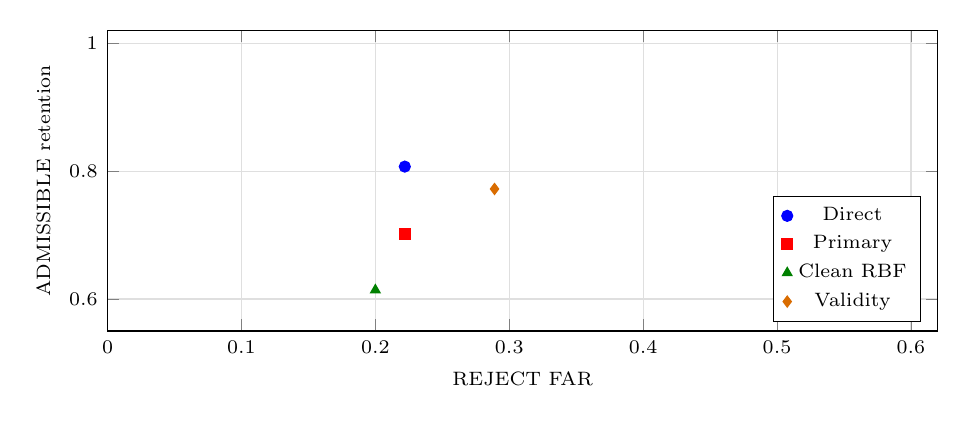
\begin{tikzpicture}
\begin{axis}[
  width=\columnwidth, height=5.4cm,
  xmin=0, xmax=0.62, ymin=0.55, ymax=1.02,
  xlabel={REJECT FAR}, ylabel={ADMISSIBLE retention},
  grid=major, major grid style={draw=gray!25},
  legend style={font=\scriptsize, at={(0.98,0.03)}, anchor=south east},
  tick label style={font=\scriptsize}, label style={font=\scriptsize}
]
\addplot[only marks, mark=*, mark size=2pt, blue] coordinates {(0.222,0.807)}; \addlegendentry{Direct}
\addplot[only marks, mark=square*, mark size=2pt, red] coordinates {(0.222,0.702)}; \addlegendentry{Primary}
\addplot[only marks, mark=triangle*, mark size=2pt, green!50!black] coordinates {(0.200,0.614)}; \addlegendentry{Clean RBF}
\addplot[only marks, mark=diamond*, mark size=2pt, orange!85!black] coordinates {(0.289,0.772)}; \addlegendentry{Validity}
\end{axis}
\end{tikzpicture}

  \caption{D2 operating points. Lower FAR and higher Retention are desirable, but coverage is a separate dimension shown in Table~\ref{tab:main-results}.}
  \label{fig:tradeoff}
\end{figure}

\subsection{Failure modes are part of the result}

The D2 run produced 93 OK, 6 INVALID\_SPANS, and 3 INVALID\_JSON generations. There were no retrieval or reranking failures. For Primary, 16 items had no candidate, 4 had invalid spans, and 3 had invalid JSON, leaving 79 valid scores. Thus 23/102 items failed before a complete Primary admission score existed. A score-only table that removed these items would report a different task than the one an event organization system must execute.

\begin{table}[t]
\centering
\caption{Primary failure accounting on D2.}
\label{tab:failures}
\small
\begin{tabular}{@{}lr@{}}
\toprule
Status & Items \\
\midrule
Valid score & 79 \\
No candidate & 16 \\
Invalid spans & 4 \\
Invalid JSON & 3 \\
Total & 102 \\
\bottomrule
\end{tabular}
\end{table}

\section{Analysis and Discussion}
\label{sec:discussion}

\subsection{What the benchmark changes}

The benchmark changes the object of comparison. A ranking model is not evaluated only by how it orders rows with a score; it is evaluated as a chain whose coverage and failure states affect the downstream action. This is why a complete-coverage direct baseline can be informative even when it is not uniformly better. It provides a reference for the cost of adding an upstream candidate-dependent signal and prevents conditional AUC from being interpreted as end-to-end admission quality.

The results also clarify why the original phenomenon is not solved by renaming \reject{} as NIL. A NIL outcome can mean that a coherent event exists but is not in the current knowledge base. Our \reject{} state means that the item is not admitted under the current organization policy. These states may require different downstream actions: clustering or knowledge-base expansion for NEW, versus stopping the item before event organization for \reject{}.

\subsection{Calibration transfer, not a leaderboard race}

The controlled EVAL60 results suggested a joint-signal advantage, but D2 did not reproduce a stable advantage. We do not interpret this as evidence that joint signals are useless. It is evidence that development-stage discrimination is not sufficient to establish a reliable admission policy under a new time window. Coverage, parser behavior, class composition, and the retention--FAR operating point all participate in the transfer.

This is precisely the kind of finding that a diagnostic benchmark should preserve. The protocol allows a future method to improve the result, but it does not allow a method to hide missing candidates or choose a threshold after seeing the challenge labels. A stronger model can be evaluated under the same contract without changing the task definition.

\subsection{Why the direct baseline does not make the task trivial}

Direct admission has a strong D2 AUC, but it still trades 46/57 retained \admissible{} items for 10/45 false \reject{} admissions at the frozen threshold. The task is therefore not reduced to the statement that one classifier is inaccurate. The benchmark asks whether a complete pipeline can make an operational decision while exposing the coverage and failure costs that a score-only binary classifier would omit. If a future simple classifier solves the policy, the protocol remains useful: it records that the task is solvable without claiming an unnecessary architecture.

\subsection{Scope and limitations}

D2 comes from one public platform, one six-day time window, and 12 fixed English topic queries. It is a challenge confirmation set rather than a probability sample. The benchmark does not estimate Web prevalence, deployment cost, or downstream harm. The P0, DEV/EVAL, and D2 materials have different evidence statuses and must not be reported as one homogeneous Gold pool. The adjudication record discloses limited machine-translation assistance. Finally, the present paper evaluates item-level admission; complete EXISTING/NEW/REJECT linking and multimodal evidence are future extensions, not completed claims.

\balance
\section{Conclusion}
\label{sec:conclusion}

Open-web event organization begins one decision earlier than conventional event linking assumes. A candidate can be retrieved without making the whole item admissible, and a system can lose an item before it produces a score. We turned this observation into a coverage-aware, unit-aware diagnostic benchmark that separates mention, target, and item; keeps development and challenge evidence distinct; and reports Retention, \reject{} FAR, coverage, and named failures together.

The frozen evaluation does not support a claim that the joint Primary system is a generally superior admission model. That negative result is part of the contribution: a development-stage signal gain did not establish a stable time-window gain, while 23/102 Primary items failed to reach a complete score. The resulting benchmark makes this calibration and measurement gap visible and reproducible. It offers a compact contract for evaluating future open-world event admission systems without conflating retrieval, linking, and downstream organization.

\section*{Data and code availability}

The authors plan to release the benchmark specification, evaluation runner, anonymized derived metadata where licensing permits, and the scripts used to reproduce the reported tables and figures. Private source posts, annotator identities, and restricted raw materials will not be released. The release will preserve the evidence hierarchy and the distinction between development, controlled diagnostic, and challenge confirmation data.

\section*{Acknowledgements}
\todo{Add acknowledgements only after the anonymous review version is finalized.}

\bibliographystyle{elsarticle-harv}
\bibliography{references}

\end{document}
